\documentclass{article}
\usepackage[utf8]{inputenc}
\usepackage{hyperref}
\usepackage{tabto}
\usepackage{graphicx}
\usepackage[export]{adjustbox}
\usepackage{xcolor}

\title{EE5121 Convex Optimization Term Paper }
\author{Adithya Swaroop}
\date{EE17B115}

\begin{document}
\maketitle

\textcolor{red}{\textbf{Title :}} Cubic Discrimination \\

\textcolor{red}{\textbf{Reference :}} Classification, Section 8.6 of the book "Convex Optimization" by Stephen Boyd and Lieven Vandenberghe (Page No: 422) \\

\textcolor{red}{\textbf{Dataset Link :}} \href{https://www.kaggle.com/kalinin84/2d-datasets-classification}{2d datasets (classification)}\\

\textcolor{red}{\textbf{Contributions :}}
\begin{itemize}
    \item Implemented the idea of Support Vector Machine into Quadratic Discrimination 
    \item Implemented Cubic Discrimination
    \item Used SVM idea to do Multi-classification (More than 2 classes classification)
    \item Applied all above classifiers on a kaggle dataset.
\end{itemize}

\newpage

\section{Robust Linear Discrimination}
\textbf{Contribution : } Applied this to kaggle 2d classification dataset.
\begin{verbatim}
cvx_begin
    variables p(2) q  t;
    maximize t;
    subject to
    x*p - q >= t;
    y*p - q <= -t;
    norm(p, 2) <= 1;
cvx_end
\end{verbatim}
\begin{figure}[h!]
    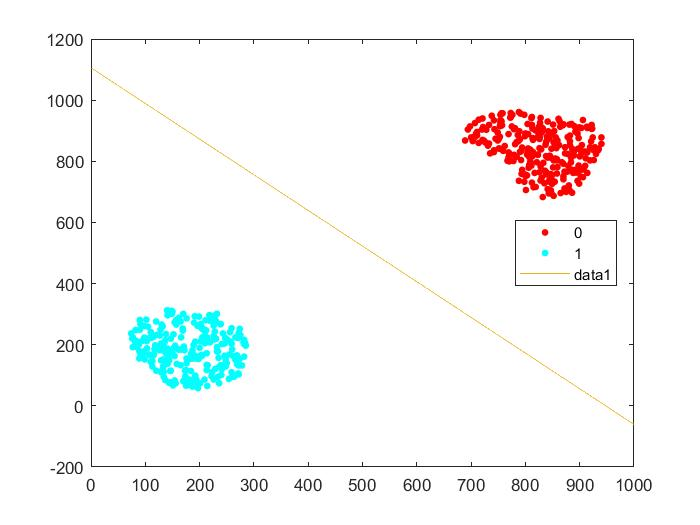
\includegraphics[width=0.7\textwidth, center ]{data1.jpg}
\end{figure}
However this thing fails in case of non-linear seperable datasets. We need to use Support Vector Machines.

\newpage
\section{Support Vector Machine classifiers}
\textbf{Contribution : } Applied this to kaggle 2d classification dataset.
\begin{verbatim}
cvx_begin
    variables u(size(x,1)) v(size(y,1));
    variables p(2) q  ;
    minimize sum(u(:)) + sum(v(:));
    subject to
        x*p - q >= 1 - u;
        y*p - q <= -(1 - v);
        u >= 0;
        v >= 0;
cvx_end
\end{verbatim}
\begin{figure}[h!]
    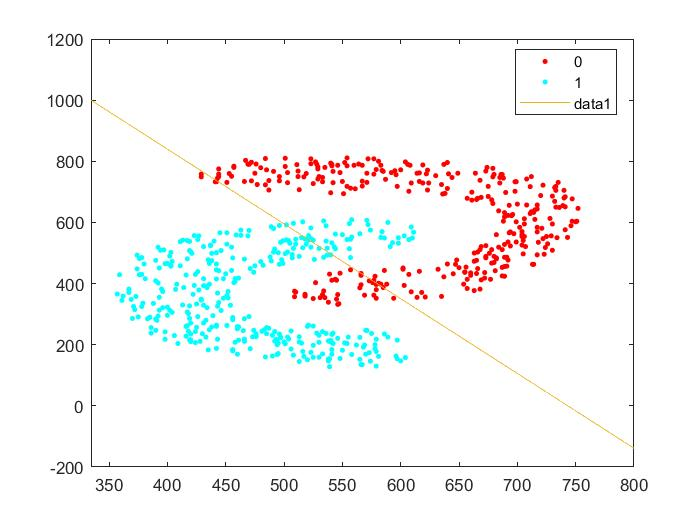
\includegraphics[width=0.7\textwidth, center ]{data2.jpg}
\end{figure}
Basically what we are trying to do is to minimize number of misclassified points. But we still couldn't get a nice boundary to classify them and it looks like a linear boundary is not going to be sufficient. So, let's try quadratic discrimination.
\newpage
\section{Quadratic Discrimination}
\textbf{Contribution:} Normal robust quadratic discrimination approach will fail because this dataset may or may not be seperated by a parabola/ ellipse. We need to use the idea of SVM here, i.e, minimize no: of misclassified points.
\begin{verbatim}
cvx_begin
    variables u(size(x,1)) v(size(y,1));
    variables c d e f g r  ;
    minimize sum(u(:)) + sum(v(:));
    subject to
        c*x(:,1).^2 + d*x(:,2).^2+ e*x(:,1).*(x(:,2))+f*x(:,1)+g*x(:,2) +r 
            >= 10-u;
        c*y(:,1).^2 + d*y(:,2).^2+ e*y(:,1).*(y(:,2))+ f*y(:,1)+g*y(:,2) +r 
            <= -(10- v);
        u >= 0;
        v >= 0;
cvx_end
\end{verbatim}
\begin{figure}[h!]
    \centering
    \begin{minipage}{0.45\textwidth}
        \centering
        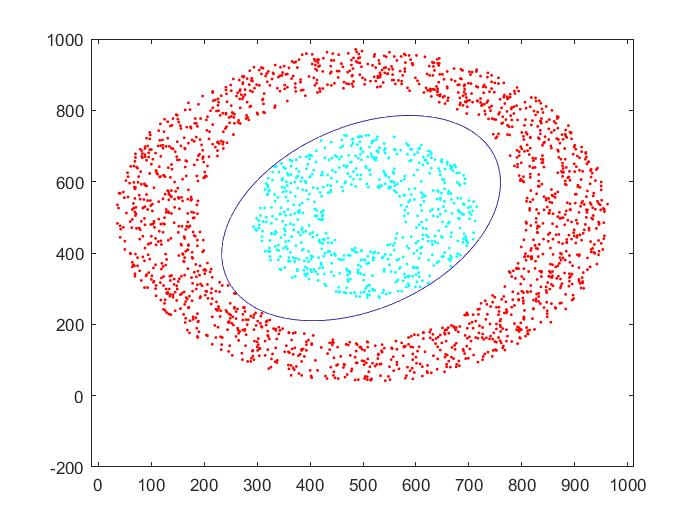
\includegraphics[width=\textwidth]{data4.jpg} % first figure itself
    \end{minipage}\hfill
    \begin{minipage}{0.45\textwidth}
        \centering
        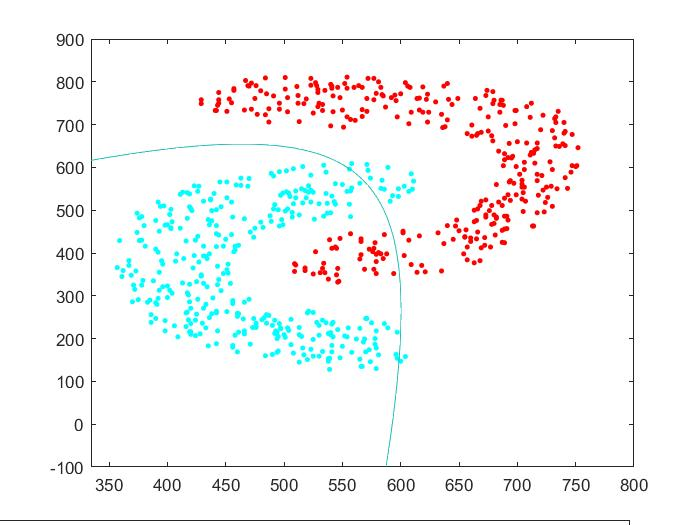
\includegraphics[width=\textwidth]{data3.jpg} % second figure itself
    \end{minipage}
\end{figure}
In first case, quadratic discrimination yields a nice boundary. But for second case, still it looks like quadratic boundary is unsufficient as the data can't be seperated by a parabola or ellipse. So, let's try Cubic Discrimination.

\newpage
\section{Cubic Discrimination}
\textbf{Contribution:} Implemented this also similar to how an SVM works and applied it to a 2d classification dataset.
\begin{verbatim}
cvx_begin
    variables u(size(x,1)) v(size(y,1));
    variables c d e f g r h k p q ;
    minimize sum(u(:)) + sum(v(:));
    subject to
        c * x(:,1).^2 + d * x(:,2).^2+ e*x(:,1).*(x(:,2)) + f *x(:,1) + g * x(:,2) + 
            h * x(:,1).^3 + p * x(:,2).^3+ q*x(:,1).*(x(:,2)).*x(:,1) + 
            k*x(:,1).*(x(:,2)).*(x(:,2)) + r >= 10 - u;
        c*y(:,1).^2 + d * y(:,2).^2+ e*y(:,1).*(y(:,2)) +  f *y(:,1) + g * y(:,2)
            +h * y(:,1).^3 + p * y(:,2).^3+ q*y(:,1).*(y(:,2)).*y(:,1) + 
            k*y(:,1).*(y(:,2)).*(y(:,2)) + r <= -(10- v);
        u >= 0;
        v >= 0;
cvx_end
\end{verbatim}
\begin{figure}[h!]
    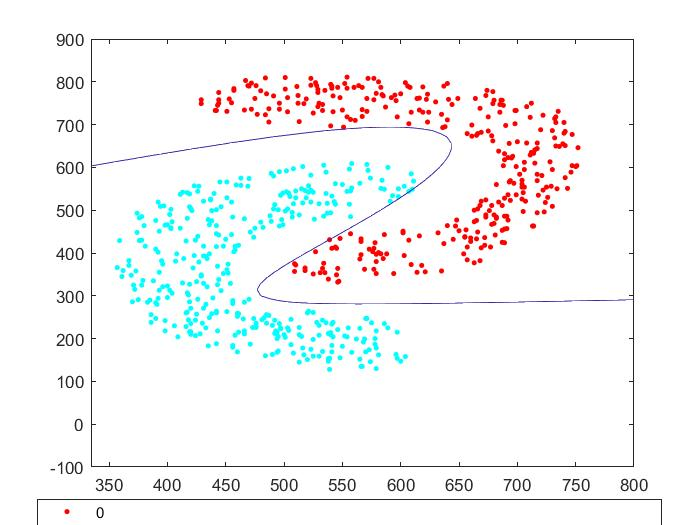
\includegraphics[width=0.7\textwidth, center ]{data5.jpg}
\end{figure}

\newpage
\section{Multi Classification}
\textbf{Contribution:} Used one vs all method to classify data into more than 2 classes in CVX. In one-vs-All classification, for the N-class instances dataset, we have to generate the N-binary classifier models. For classifying the object to class 1, we need to linearly seperate class 1 objects and objects of classes other than class 1, similarly N times for N classes.
\begin{verbatim}
cvx_begin
    variables u(size(x,1)) v(size(y,1)) w(size(z,1));
    variables p(2) q  ;
    minimize sum(u(:)) + sum(v(:)) + sum(w(:));
    subject to
        x*p - q >= 1 - u;
        y*p - q <= -(1 - v);
        z*p - q <= -(1 - w);
        u >= 0;
        v >= 0;
        w >= 0;
cvx_end
  
cvx_begin
    variables u(size(x,1)) v(size(y,1)) w(size(z,1));
    variables p(2) q  ;
    minimize sum(u(:)) + sum(v(:)) + sum(w(:));
    subject to
        y*p - q >= 1 - v;
        x*p - q <= -(1 - u);
        z*p - q <= -(1 - w);
        u >= 0;
        v >= 0;
        w >= 0;
cvx_end
    
cvx_begin
    variables u(size(x,1)) v(size(y,1)) w(size(z,1));
    variables p(2) q  ;
    minimize sum(u(:)) + sum(v(:)) + sum(w(:));
    subject to
        z*p - q >= 1 - w;
        x*p - q <= -(1 - u);
        y*p - q <= -(1 - v);
        u >= 0;
        v >= 0;
        w >= 0;
cvx_end
\end{verbatim}
\begin{figure}[h!]
    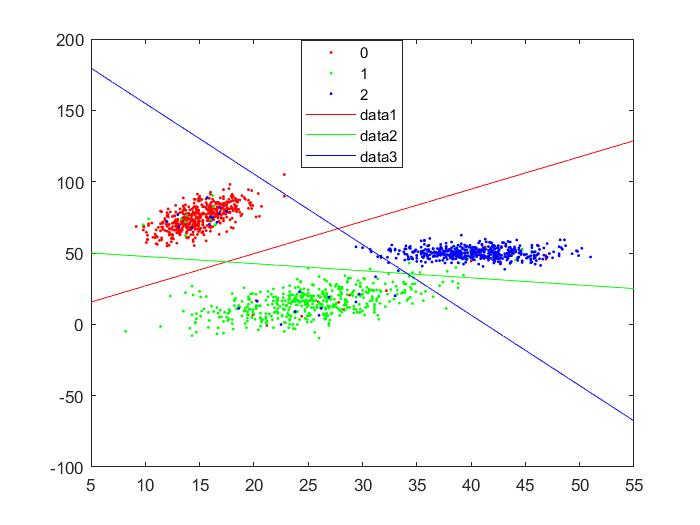
\includegraphics[width=0.7\textwidth, center ]{data6.jpg}
\end{figure}
Here, blue line seperates blue points from others, red line seperates red points from others and green line seperates green points from others.



\end{document}
